\documentclass[11pt, titlepage]{article}
\usepackage{beamerarticle}
\usepackage[utf8]{inputenc}
\usepackage{hyperref}
\usepackage{amssymb,amsmath}

% Page settings
\usepackage[letterpaper, margin=1in]{geometry}
%\usepackage{palatino}%\usepackage{lmodern, times}
\usepackage{lmodern}%\usepackage{lmodern, times}
\usepackage{setspace}                           
\onehalfspacing %\doublespacing  % \singlespacing 

% Appendix
\usepackage{appendix}

% Line numbers
%\usepackage{lineno}
%\linenumbers


% Tables
\usepackage{array,booktabs,longtable,rotating}
\newenvironment{tablenotes}[1][]{
  \begin{minipage}{\textwidth}\emph{Notes:}{\footnotesize #1}
}{\end{minipage}}
\makeatletter
\def\fps@table{htbp}
\makeatother

% Graphics
\usepackage{graphicx,grffile}
\makeatletter
\def\maxwidth{\ifdim\Gin@nat@width>\linewidth\linewidth\else\Gin@nat@width\fi}
\def\maxheight{\ifdim\Gin@nat@height>\textheight\textheight\else\Gin@nat@height\fi}
\makeatother
% Scale images if necessary, so that they will not overflow the page
% margins by default, and it is still possible to overwrite the defaults
% using explicit options in \includegraphics[width, height, ...]{}
\setkeys{Gin}{width=\maxwidth,height=\maxheight,keepaspectratio}
% set default figure placement to htbp
\makeatletter
\def\fps@figure{htbp}
\makeatother

\usepackage{natbib}% plainnat
\bibliographystyle{abbrvnat}
\setcitestyle{authoryear,open={(},close={)}}
%\bibliographystyle{aer}


\setlength{\emergencystretch}{3em}  % prevent overfull lines
\providecommand{\tightlist}{%
  \setlength{\itemsep}{0pt}\setlength{\parskip}{0pt}}



\institute{}
\titlegraphic{}

\usepackage{xcolor}
\newcommand\todonote[1]{\textcolor{red}{#1}}



% Subscript
\newcommand\sub[1]{_{#1}}
\newcommand\supsc[1]{^{#1}}

\title{Incentives for Public Goods Inside Organizations: Field Experimental
Evidence\thanks{Blasco: Harvard Institute for Quantitative Social Science, Harvard
University, 1737 Cambridge Street, Cambridge, MA 02138 (email:
\href{mailto:ablasco@fas.harvard.edu}{\nolinkurl{ablasco@fas.harvard.edu}}).
Jung: Harvard Business School, Soldiers Field, Boston, MA 02163 (email:
\href{mailto:ojung@hbs.edu}{\nolinkurl{ojung@hbs.edu}}), Lakhani:
Harvard Business School, Soldiers Field, Boston, MA 02163, and National
Bureau of Economic Research (email:
\href{mailto:k@hbs.edu}{\nolinkurl{k@hbs.edu}}). Menietti: Harvard
Institute for Quantitative Social Science, Harvard University, 1737
Cambridge Street, Cambridge, MA 02138 (email:
\href{mailto:mmenietti@fas.harvard.edu}{\nolinkurl{mmenietti@fas.harvard.edu}}).
We gratefully acknowledge the financial support of the MacArthur
Foundation (Opening Governance Network), NASA Tournament Lab, and the
Harvard Business School Division of Faculty Research and Development.
This project would not have been possible without the support of Eric
Isselbacher, Julia Jackson, Maulik Majmudar and Perry Band from the
Massachusetts General Hospital's Healthcare Transformation Lab.}}
\author{Andrea Blasco \and Olivia S. Jung \and Karim R. Lakhani \and Michael Menietti}
\date{Last updated: 27 March, 2017}

\begin{document}
\maketitle
\begin{abstract}
Employees often make choices between working on their assignment and on
opportunities to improve the organization for the benefit of others.
Inefficient decisions may arise due to an incentive to free-riding on
the work of others. An internal competition for prizes may help workers
make more efficient choices but it may be detrimental to motivated
workers. Using a solicitation of innovation project proposals in a
medical center with over 1200 employees, we find that a contest awarding
pecuniary prizes for the best contributions generates an 85 percent (2.5
percentage points) increase in participation, with no effects on the
quality of contributions. The participation effect is the same for men
and women, staff with different roles, and appears~beyond the value of
the prize. We also find that a solicitation appealing to improving the
workplace is also effective. However, emphasizing the mission of the
organization led to countervailing effects on participation based on
gender differences. These results indicate that awarding prizes is a
powerful way to foster contributions to organizational public goods,
suggesting a complementarity between incentives and underlying
motivations associated with the mission of the organization.

\smallskip\noindent 
JEL Classification: H41; D23; D03.

\smallskip\noindent 
Keywords: innovation contest; free rider problem; social preferences; altruism; idea generation; organization of work.
\end{abstract}


% Todo notes
%\usepackage[textsize=tiny]{todonotes}
%\newcommand\redmarginpar[1]{\marginpar{\footnotesize{\textcolor{red}{#1}}}}
%\listoftodos[Notes]
\clearpage

\section{Introduction}\label{introduction}

Inside organizations, employees often make choices between working on
their regular assignment and developing opportunities to improve the
workplace. For example, a worker may concentrate on production tasks
alone -- with pay and promotion tied to performance in these activities
-- or also devote time and energy to solve common organizational
problems -- with no direct compensation for the worker. This situation
leads to two key issues in the analysis of incentives inside
organizations. First, there is a problem of designing compensation
schemes for employees to take the correct actions by addressing any
potential \emph{multitasking} issue
\citep{holmstrom1991multitask, hellmann2011incentives, manso2011motivating}.
Second, there is a \emph{public good contribution} problem. Because of
the non-rival nature of work that benefits the organization as a whole,
employees may be tempted to avoid working on these tasks in the hope to
free-ride on the efforts of others.

An internal competition for prizes, such as a promotion or a bonus, is
often viewed as a proper way to provide incentives in such situations.
Contests can stimulate risk taking and participation in less-easily
contractible tasks, as discussed by \citet{lazear1981rank};
\citet{green1983comparison}; \citet{mary1984economic} among others.
However, traditional organizational literature does not take into
account the non-rival nature of contributing which constitutes the
public good problem. Standard contest theory models presumes that the
contest outcomes will be enjoyed only by the sponsor of the competition
(e.g., the manager, entrepreneur) with small gains for the competitors
beyond the prizes given to the winners.\footnote{One notable exception
  is the model of tournaments with positive externalities introduced by
  \citet{drago1988incentive}.} Though realistic in many situations, this
assumption becomes questionable when competitors can expect gains from
the work of others, as in the case of a competition aiming at
organizational improvements. The use of contests under these
circumstances raises an important question: Will prizes be effective in
fostering participation and contributions to internal public goods
inside organizations?

In the present study, we report the results of a natural field
experiment to compare two dominant perspectives on the issue. The first
comes from the seminal work of \citet{morgan2000financing}, who stresses
that awarding prizes in lottery-like contests will mitigate, or even
eliminate, the incentive to free riding. At the margin, employees choose
their effort levels so that expected gains and costs are equal. Because
these gains include the direct utility from receiving personal rewards
and from improving the organization, even small prizes will boost
participation beyond what one would expect from the pecuniary value of
the prize alone. The second perspective is that, when the task matches
the preferences of workers in increasing organizational efficiency,
workers will volunteer their effort and organizations can economize on
the incentives, as discussed by \citet{besley2005competition},
\citet{prendergast2007motivation}, \citet{delfgaauw2008incentives} among
others.\footnote{Everyday evidence for this kind of ``altruistic''
  behavior comes from blood donations, charitable giving, social
  workers. See also the results of laboratory experiments based on
  economic games \citep[see][]{levitt2007laboratory} and field studies
  showing evidence on prosocial preferences at work
  \citep{bandiera2005social, dellavigna2016estimating}.} Furthermore,
announcing a competition for prizes can also cause unintentional adverse
consequences. It may evoke mixed feelings in workers with different
competitive inclinations or risk aversion, a disposition potentially
different for men and women \citep{niederle2007women, croson2009gender};
it may inadvertently promote unethical behavior
\citep{lazear1989pay, charness2013dark}; weaken intrinsic motivations
\citep{reeve1996elements, frey1997not}; and even kill the creativity of
innovative work \citep{erat2015incentives}.

The study was conducted in collaboration with the Massachusetts General
Hospital's (MGH) Corrigan Minehan Heart Center (``Heart Center''), a
prominent medical organization in the United States and a teaching
hospital of the Harvard Medical School. The health care delivery context
is particularly relevant for studying public-good provision problems as
the need for organizational improvement and innovation is vastly noted
\citep[e.g.,][]{cutler2012reducing}. Also, health care professionals are
commonly seen as motivated workers willing to step beyond the boundaries
of their contractual duties to offer better care
\citep{delfgaauw2005dedicated}, which makes the comparison of different
incentives in a public good context particularly relevant.

The context of the experiment was the launch of an internal four week
``innovation contest'' aimed at improving the operations of the
organization, in the spirit of ``open innovation'' initiatives discussed
in \citet{terwiesch2008innovation}, \citet{guinan2013experiments},
\citet{lakhani2013prize}, and \citet{glaeser2016predictive}. Employees
were asked to submit project proposals addressing existing problems or
providing improvements. The MGH executives committed to giving top
proposals proper resources for implementation. Staff members could
expect more costs and responsibilities from making a winning proposal,
such as providing further guidance or a direct involvement in special
implementation teams. These other costs were not well matched by any
direct compensation from winning the competition. Employees having made
the top submissions were awarded in-kind prizes (Apple iPad mini's), the
value of which was relatively small in comparison to the foreseeable
costs of unpaid project implementation time.

The subject pool was the entire population of over 1,200 staff members
of the Heart Center including physicians, nurses, and administrative
workers. Our main intervention was in altering the content of
personalized solicitations to participate in the innovation contest
among randomly selected staff members. By doing so, we were able to get
causal estimates of the effect of different incentives on two main
outcomes: (a) the decision to submit and engage in implementation
activities of a project proposal and (b) the quality of the proposal
submitted, as measured by over 12,000 ratings made by peers. Using data
on profession and gender, we could also characterize the heterogeneity
of responses to the treatment, testing the implications of our
intervention for the organization.

We designed four treatments related to our research questions. In a
first treatment (PRIZE), the solicitation nudged employees to
participate in the initiative by announcing a personal reward (an Apple
iPad mini) for the top submissions. In a second treatment (FUND), the
solicitation nudged employees with the funding opportunity alone and an
explicit commitment by Hearth Center executives to pay expenses up to
\$20,000 towards implementation of the proposal (the submitters would
not receive this money for personal use). In the remaining two
treatments, we ``framed'' the contest by emphasizing the opportunity to
improve the healthcare of the patients (PCARE) or the workplace
(WPLACE).

We find that workers were eager to contribute to improving the
organization despite its cost: 196 employees (16 percent) across the
entire organization took part in the initiative, with 5 percent of our
sample submitting project proposals.\footnote{By comparison, in a purely
  public good setting such as \citet{list2002effects}'s field experiment
  on individual monetary contributions to charity, the authors find very
  similar participation rates between 3 and 8 percent. Similarly, in a
  setting that involves employees of a consulting company making
  proposals to clients with no clear public good incentive,
  \citet{gibbs2014field} finds participation rates that are slightly
  higher (about 10 percent) but over a two-year period versus our
  four-week competition.} About half of these participating employees
were invited by Heart Center executives to follow up with detailed
implementation plans, which culminated in two proposals receiving full
funding.

Our main finding is that small prizes boosted participation without
lowering the quality of the submissions. In fact, simply announcing a
personal reward (PRIZE) produced a 2.5 percentage points (85 percent)
increase in participation rates than the average. This effect appears
too large to fit a pure contest environment without public good
incentives. The relatively high incomes of our subject pool, the low
chance of winning, and the additional costs of being selected for
implementation suggest that very few would find it advantageous to
participate. We discuss several possible explanations for this
observation. We conclude that awarding a prize increased participation
by helping employees internalize the effects of their active
participation for improving the organization, as in
\citet{morgan2000financing}. We then use a simple model to estimate the
employees' underlying preferences for the public good, showing that
these preferences can account for 25 percent of individual costs of
submitting.

Analysis of the ratings received by the proposals indicates there was no
crowding-out effect, as the higher propensity of workers in the prize
treatment does not seem to be driven by low-quality submissions. This
result is robust to using ratings from the contest organizers instead of
those from peers. We also find little evidence of a difference in
content other than peer-evaluated quality, such as the count of projects
proposals per proponent, the areas of focus, and the proposal length.
Overall, these findings suggest no negative trade-off between quantity
and quality: treatments that attracted more participants resulted in
proposals of comparable quality and content. This also implies that
monetary incentives were not counter-productive to creativity compared
to voluntary contributions.

We did, however, find that a framing around the mission of the
organization resulted in responses that were sensitive to the gender of
the solicited person. Women's participation was greater when emphasizing
the patient care mission (PCARE) whereas men's participation was
significantly lower, controlling for the profession. At the same time,
we do not find gender-based differences with respect to participation in
the prize (PRIZE) treatment: women's participation was slightly higher
(but not significant) than men's. The first finding suggests that female
workers may perceive the mission of the organization differently than
male workers. Alternatively, women workers were simply more responsive
to a call for helping patients probably due to gender-based
self-stereotyping. The second evidence indicates relatively small and
inconsequential gender difference in preferences such as competitive
inclinations or risk aversion between men and women.

Finally, announcing a funding opportunity alone (FUND) -- even with a
commitment of \$20,000 in project funding -- made employees less likely
to submit compared to all other treatments and no difference in the
quality of submissions. This evidence confirms that to being in charge
of the (winning) project was not perceived as a prize in itself. Hence,
soliciting participation in this task without a proper announcement of
personal rewards for the winners or the right framing might have
exacerbated the incentives to free-riding.

\section{Literature}\label{literature}

The present study contributes to the literature on the use of prizes
(relative incentives) in the workplace \citep[among
others]{lazear1981rank, green1983comparison, mary1984economic}. Our main
contribution consists in studying the role of prizes in fostering
workers' participation in the field and in activities that produce
organizational improvements. In particular, the observed increase in
participation in the PRIZE treatment is consistent with the results of
existing empirical studies
\citep{bull1987tournaments, knoeber1994testing, eriksson1999executive, ehrenberg1990tournaments, terwiesch2008innovation, terwiesch2009innovation, boudreau2011incentives, boudreau2016performance}.
However, while most studies focus on tournaments that result in benefits
enjoyed exclusively by the sponsor of the competition (increasing sales,
production, revenues), we show that this positive result generalizes to
situations that generate positive externalities for the contestants
(innovation projects to improve the organization). Despite being a
common situation,\footnote{Members of the same organization often end up
  competing on the basis of their ability to solve common issues at the
  organizational level, such as addressing specific problems,
  innovating, providing business ideas.} this setting has received
relatively less attention in past studies.

Our work also contributes to the empirical literature on the use of
contest-type lotteries to finance public goods that was first studied by
\citet{morgan2000financing}. A number of works have shown a positive
effect of prizes on the extent of individual contributions to a public
good in the laboratory
\citep{morgan2000funding, dale2004charitable, lange2007using} and in the
field \citep{landry2006toward}. However, as noted by
\citet{vesterlund2012voluntary}, the existing evidence on the
profitability of contest-type mechanisms for raising money for public
goods (e.g., charity donations) is only mixed
\citep{vesterlund2012voluntary}. Our work provides further evidence to
this theory as we generalize the results of past studies to an
organizational setting. Within this setting, individual contributions
are non-monetary but consist of time and effort in putting forward (and
implementing) a proposal. Whereas the public good consists of the
potential improvements for the organization. Under such circumstances,
we find evidence indicating that prizes can be very effective tools for
raising the level of participation (compared to voluntary mechanisms)
and appear overall a profitable solution for organizations.

Our results also relate to the literature on social preferences at work.
A number of studies have shown that people tend to contribute to public
goods despite strong incentives to free ride. According to the World
Health Organization, about 60 percent of blood donations collected
globally each year is from voluntary unpaid blood donors. According to
\citet{list2011market}, charitable gifts of money are worth 2 percent of
gross domestic product for the United States.
\citet{lacetera2014rewarding} stresses that: ``27\% of Americans
volunteer with formal organizations, for a total of about 8 billion
hours per year.'' A sizable scientific evidence on this topic comes from
a series of studies based on economic games in the laboratory
\citep[see][ for a review]{levitt2007laboratory} and in the field
\citep{bandiera2005social, dellavigna2016estimating}.
\citet{bandiera2005social}, for instance, shows that workers internalize
preferences of co-workers and may reduce effort under relative
incentives. Likewise, \citet{dellavigna2016estimating} shows a positive
effect of mission-oriented preferences, also called ``vertical social
preferences,''\footnote{Social preferences towards peers are instead
  called ``horizontal.''} on the level of effort of freelance workers
folding envelopes for a charity. Our work is consistent with a positive
effect of vertical social preferences; adding evidence that such social
preferences not only increase effort in mandatory pre-specified tasks
but also affect voluntary participation to non-mandatory ones.\footnote{In
  \citet{dellavigna2016estimating}, workers can choose how much effort
  to exert but cannot choose which task to work on (in this sense the
  task is ``mandatory'').}

Another important aspect of the present study is that we focus on
incentives to carry out a complex task (writing a project proposal) as
opposed to standardized production tasks \citep{knoeber1994testing} or
sport \citep{ehrenberg1990tournaments}. We also focus on a competition
among individual workers instead of teams
\citep[e.g.,][\citet{hamilton2003team} and more recently
\citet{gibbs2014field}]{erev1993constructive}. This allows us to remove
from consideration important team dynamics such as peer pressure,
monitoring, reciprocity within the team that may also affect the
participation and effort quality of employees.

Finally, our work provides support to the incentive effect of a personal
satisfaction derived from helping the organization achieving its goals
\citep{akerlof2005identity, besley2005competition, delfgaauw2005dedicated, delfgaauw2008incentives, prendergast2007motivation}.
This type of altruism is believed to be an important driver of effort
for workers in organizations for social public goods, such as hospitals,
universities, schools, administrations, and the military. Theoretical
models suggest different ways in which managers can exploit these
prosocial motivations to raise individual productivity; in the current
study, we use ``framing'' to make particular motivations salient. We
find that emphasizing prosocial motivations has countervailing effects
on participation; negative for men and positive for women.\footnote{Concerning
  framing, many studies have explored the effects of positive or
  negative framing on the private provision of public goods in the
  laboratory \citep{andreoni1995warm}. Inside organizations,
  \citet{hossain2012behavioralist} and \citet{hong2015framing} are among
  the first studies to measure the impact of framing interventions on
  productivity. The current study adds to this literature by showing
  significant effects associated with a particular type of framing such
  as appealing to internal motivations towards the mission of the
  organization.} While this finding is consistent with altruism being
one important driver of effort inside organizations, it also suggests
that people are sensitive to framing and in ways that may be difficult
to predict ex-ante.

\section{Analytical framework and
predictions}\label{analytical-framework-and-predictions}

In this section, we conceptualize an internal solicitation for
innovation project proposals to improve the operations of the
organization as a voluntary contribution mechanism for a public good.
Successful proposals are viewed as non-excludable because innovation
leads to improvements for everyone in the workplace (including customers
by increasing the quality and efficiency of the services provided).
Submitting a proposal requires costly effort by employees, such as the
time to identify a problem, form a proposal, write up a concise
description, and the potential for further involvement during proposal
implementation.

Consider a linear model of the utility of a typical employee who
contributes \(x\) and benefits from total contributions of \(Y=\sum x\):

\begin{equation} \label{eq:utility}
  u(R,~ Y) =  \gamma Y + \delta x + \frac{x}{Y} R - c x.
\end{equation}

The benefits of contributing derive from three sources. First, there is
an altruistic benefit from the improved workplace, \(\gamma Y\). The
altruistic benefits are the crux of public goods. Only the existence of
an improved workplace is desired and the source of contributions is
irrelevant. Thus, everyone would prefer to free-ride on others' efforts.
Second, participants have some chance of winning the contest and can
expect to derive benefits from the prizes, \(\frac{x}{Y} R\), where, for
simplicity, all efforts have an equal chance of being selected as the
winner, as in \citet{morgan2000financing}. The personal reward \(R\) can
be thought of as a pecuniary prize, but it could also be an increase in
prestige or recognition or any combination of the above. Finally,
employees may have an egoistic motivation for contributing ``per se,''
regardless of winning and the effect on others, which is captured by
\(\delta x\). This includes also the case in which workers may derive a
personal satisfaction from contributing personally to the organization,
often called warm glow preferences for giving \citep{andreoni1995warm}.
Since we cannot observe the distinction between altruistic and warm-glow
motives in our empirical setup, we are going to impose later that these
preferences are such that \(\delta=0\).

Contributors incur some effort cost from developing and submitting a
proposal, \(c x\). If there are \(n\) employees the public goods dilemma
arises when \(\gamma+\delta < c < n\gamma+\delta\). Then no individual
would contribute without a reward as costs exceed individual benefits,
but everyone would be better off if everyone contributes.

Suppose contributing a proposal is a discrete choice by employees. An
employee can either contribute a single proposal \(x=1\) and receive
utility of

\begin{equation}
  u_1 = \gamma \hat Y + \delta + \sum_{k=1}^{n}\Pr(Y=k)\frac{R}{k}  - c, 
\end{equation}

where \(\hat Y\) denotes the expected level of contributions and
\(\Pr(Y=k)\) is the probability of having \(k\) total contributions. Or
they can contribute nothing \(x=0\) and receive utility of

\begin{equation}
  u_0 = \gamma (\hat Y - 1).
\end{equation}

If there are \(n\) employees, then the unique symmetric mixed-strategy
equilibrium is for each employee to contribute a proposal with
probability \(p>0\). After using the binomial probability for
\(\Pr(Y=k)\), the payoff-equating condition to find a mixed-strategy
equilibrium is:

\begin{equation} \label{eq: mixed-strategy}
  \frac{1- (1-p)^{n}}{n p} = (c- \gamma - \delta) / R.
\end{equation}

This equation admits one single solution \(p^*\) which cannot be
expressed explicitly. Using a first order Taylor expansion around \(p\),
the equilibrium probability can be approximated as follows:

\begin{equation} \label{eq: probability}
  p^*  \approx \frac{2 (R- c+\gamma +\delta )}{(n-1) R}. 
\end{equation}

The analysis of the above model is used to derive the following
predictions.

\begin{enumerate}
\def\labelenumi{\arabic{enumi})}
\item
  The probability of contributing a proposal to improving the
  organization is zero when the prize for winning is sufficiently small
  relative to the individual cost of effort minus the preference for the
  public good (i.e., \(R< c-\gamma +\delta\)).
\item
  The probability of contributing a proposal to improve the organization
  increases with the value of the prize for winning.
\item
  The probability of contributing a proposal to improve the organization
  increases with the extent of individual preference for the public good
  (\(\gamma+\delta\)).
\end{enumerate}

Now suppose that the public good \(Y\) constitutes the sum of innovation
projects to improve the organization. Imagine that the quality of each
project is randomly drawn from a discrete distribution, the same for
every contributor (every employee who contributes is assumed to be
equally likely to come up with a useful idea). Each proposal can be of
high quality with probability \(\nu\) and of low quality with
probability \(1-\nu\). If a proposal is of low quality, then the value
for the organization is normalized to zero. The quality of proposals is
learned only after the agent paid the cost of effort. Now the
equilibrium public good \(Y\) is not deterministic but follows a
binomial distribution with average \(E[Y] = p^{**} \nu n\), where the
equilibrium probability \(p^{**}\) can be derived as before with the
only difference being that it is also an increasing function of the
probability \(\nu\). This leads to the following prediction.

\begin{enumerate}
\def\labelenumi{\arabic{enumi})}
\setcounter{enumi}{3}
\tightlist
\item
  If the public good depends on the quality of each contribution and
  every agent is equally likely to make a proposal of high quality, then
  the higher the probability of contributing, the higher is the average
  public good.
\end{enumerate}

This framework can be extended to the case of individuals with
heterogeneous costs. In the appendix, we explicitly consider the case of
two types of individuals with different marginal costs of effort that
form two groups of equal size. The symmetric mixed-strategy equilibrium
is then characterized by the vector of probabilities of contributing
with a proposal \((p_1^\star, p_2^\star)\). Here, the analysis of the
payoff-equating conditions for the mixed-strategy equilibrium shows that
the higher the marginal cost of effort minus preference for
contributing, the lower the equilibrium probability of individuals
(i.e., \(p_1^\star > p_2^\star\) when \(c_1 < c_2\), and vice versa).
This leads the final prediction.

\begin{enumerate}
\def\labelenumi{\arabic{enumi})}
\setcounter{enumi}{4}
\tightlist
\item
  If individuals have heterogeneous costs, then the probability of
  contributing a proposal to improve the organization is higher for
  agents with lower costs (positive sorting).
\end{enumerate}

\section{Experimental Design}\label{experimental-design}

\subsection{The context}\label{the-context}

The Heart Center is a leading academic medical center specializing in
clinical cardiac care and research in the United States. Founded more
than a hundred years ago, the Heart Center serves thousands of patients
every year, occupies more than 35,000 square feet of office space, and
employs more than 1,200 people (nurses, physicians, researchers,
technicians, and administrative staff) scattered across several
buildings on the Massachusetts General Hospital's main campus in
downtown Boston and a few other satellite locations.

The study was in cooperation with the Heart Center's launch of the
Healthcare Transformation Lab (HTL), an initiative aimed at developing
innovative health care process improvements to enhance the health care
safety and delivery of the hospital.\footnote{See
  \url{http://www.healthcaretransformation.org} for more information
  about the HTL initiative.} The launch of the HTL was accompanied by
the announcement of an internal ``innovation contest,'' called the Ether
Dome Challenge (the name is taken from a historical place on MGH's main
campus where the first public surgery using anesthesia was demonstrated
in 1846) that sought to engage all staff members to participate.

The communication around the innovation contest highlighted the
opportunity for staff to help in the selection process of the ideas and
a commitment by the Heart Center Management that the leading ideas would
be provided appropriate resources so that they could be implemented. The
announcement on the contest's website read:

\begin{quote}
If you've noticed something about patient experience, employee
satisfaction, workplace efficiency, or anything that could be improved;
if you've had an inspiration about a new way to safeguard health; or if
you simply have a cost-saving idea, then now is the time to share your
idea.
\end{quote}

\begin{figure}
\centering
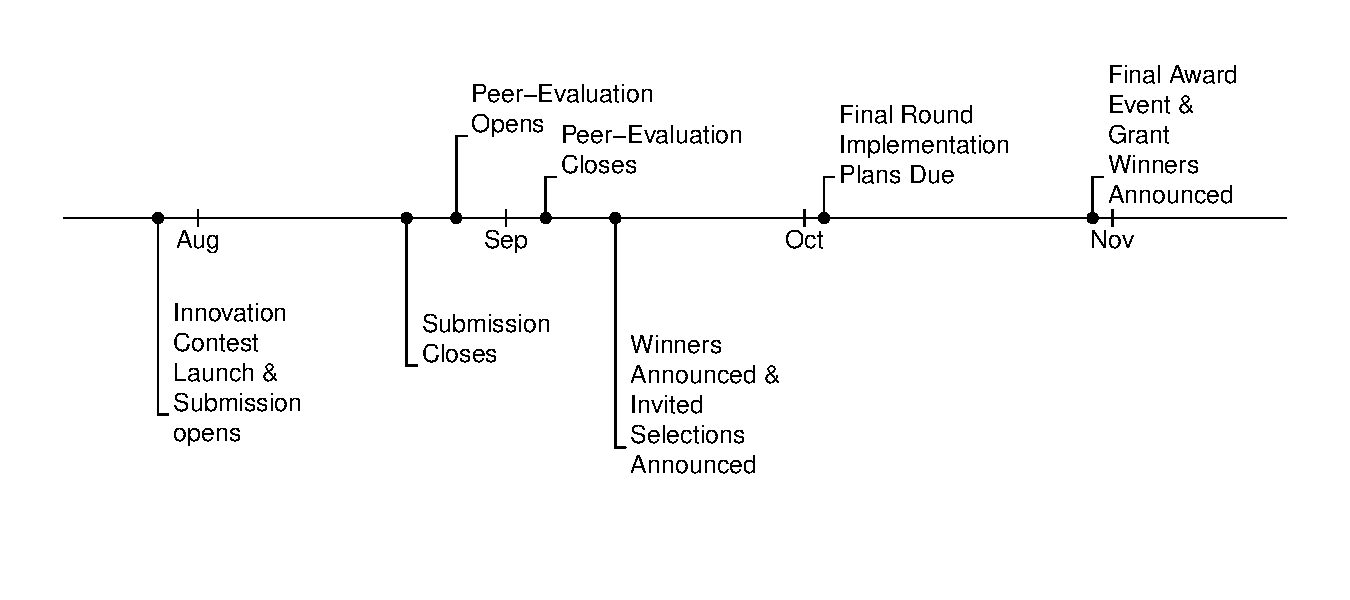
\includegraphics{Figures/timeline-1.pdf}
\caption{Timeline of the innovation contest\label{fig: phase}}
\end{figure}

The innovation contest was divided into three main phases: the
submission phase, the peer evaluation phase, and the implementation
phase. The timing is shown in Figure \ref{fig: phase}.

In the four-week submission phase, all staff members were encouraged to
identify one or more organizational problems and submit proposals
addressing them. Employee participation was voluntary. All project
submissions were done online via the website of the contest. There was
no limit to the project proposals to submit (proposals could cover any
issue within the organization, as described above), but each proposal
was limited to approximately 300 words to lower the costs of entry and
encourage broader participation. To ensure that treatment effects could
be isolated, identified, and matched to participants, team submissions
were not permitted. Limiting submissions to individual participation
allowed us to match each submitter's characteristics to the randomly
assigned treatment. It also lowered incentives to communicate or
exchange information with other employees. Also, the website was
designed to not provide any information about the status of the contest
during the submission period. In this way, decisions could not be easily
influenced by the perceived popularity of the contest or previous
submissions.

In the two-week peer evaluation phase, all staff members were invited to
rate the merit and potential of submitted proposals on a five-point
rating scale. All evaluations were done online on the website of the
contest. Each signed-up employee was shown a list of anonymized
proposals to read and rate. Proposals were presented at random in
batches of 10 each. Each proposal was described by a title, a main
description of the problem to solve, and the proposal. Voting was then
introduced by the following text: ``Rate this idea'' followed by the
rating scale: 1-low; 2; 3; 4; 5-high. Ratings were kept confidential and
the website did not provide any feedback or any other kind of additional
information that might have influenced individual judgment until the
voting phase was over. Evaluators were free to decide how many (and
which) proposals to rate. Since these were presented in a random order,
every proposal had on average the same exposure to people asked to rate
its quality. Evaluators were offered a limited edition T-shirt as a
compensation for the effort in voting.

In the final implementation phase, employees having submitted proposals
highly rated by peers and judged as particularly promising by the HTL
staff were invited to submit a full proposal detailing plans for
implementation. Following evaluation by MGH senior leadership, top
proposals were selected to receive support and funding for
implementation. This final phase took a few months to complete,
essentially the time necessary to select and implement the best
projects.

\subsection{The design}\label{the-design}

The main intervention was to alter the content of the communication that
announced the innovation contest. The start of the submission phase was
indeed announced to all staff members in a series of personalized
emails. A direct message was sent to each contact in the list of
employees' emails from our subject pool.

The body of this communication with a placeholder for our treatment is
reported below (a copy of the exact email is in the Appendix).

\begin{quote}
Dear Heart Center team member,

{[}TREATMENT HERE{]}

The Ether Dome Challenge is your chance to submit ideas on how to
improve the MGH Corrigan Minehan Heart Center, patient care and
satisfaction, workplace efficiency and cost. All Heart Center Staff are
eligible to submit ideas online. We encourage you to submit as many
ideas as you have: no ideas are too big or too small!

Submissions will be reviewed and judged in two rounds, first by the
Heart Center staff via crowd-voting, and then by an expert panel.
Winning ideas will be eligible for project implementation funding in the
Fall of 2014!
\end{quote}

The first paragraph of the above message was randomized into \emph{four}
different solicitation treatments: FUND, PRIZE, PCARE and WPLACE. Thus,
creating four treatment groups of equal size (Table
\ref{experimental-design}).

In the first two groups (FUND and PRIZE), the solicitation nudged
employees to participate by announcing individual prizes to be won
(PRIZE), i.e., an Apple iPad mini, or a \$20,000 budget for developing
their project proposals (FUND). In the remaining two groups (PCARE and
WPLACE), the solicitation ``framed'' the contest as an opportunity to
improve the healthcare of their patients (PCARE) or the workplace
(WPLACE). The exact words are in Table \ref{experimental-design}. In all
groups, employees were not told that they were part of an experiment.

\begin{table}
\centering
\caption{Experimental design}
\label{experimental-design}
\begin{tabular}{@{}lccp{10cm}}
  \\[-1.8ex]\hline \hline \\[-1.8ex]
 & \multicolumn{2}{c}{\emph{Employees:}}& \multicolumn{1}{c}{\emph{Randomized solicitation:}}\\
 \cmidrule(lr){2-3} & Obs. & \% & First paragraph \\ 
  \hline \\[-1.86ex]
PRIZE & 312 & 25 & Submit your ideas to win an Apple iPad mini \\ 
  [1.8ex] FUND & 308 & 25 & Submit your ideas to win project funding up to \$20,000 to turn your ideas into actions \\ 
  [1.8ex] PCARE & 310 & 25 & Submit your ideas to improve patient care at the Heart Center \\ 
  [1.8ex] WPLACE & 307 & 25 & Submit your ideas to improve the workplace at the Heart Center \\ 
  [1.8ex] Total & 1237 & 100 &  \\ 
   \\[-1.8ex]\hline \hline \\[-1.8ex]
\end{tabular}
\end{table}

A sample size of more than 300 units for each treatment ensured a
sufficiently high statistical power based upon standard power
calculations on the difference of proportions \citep{cohen1992power}. In
testing the difference of proportions between any two treatments, the
probability of type-I errors was slightly below \(0.80\) for
\emph{small} differences at 5 percent significance level but higher than
\(0.80\) for \emph{medium} and \emph{large} differences at the more
stringent 1 percent significance level.\footnote{The definition of
  small, medium and large differences is given by
  \citet{cohen1992power}; e.g., a difference of 5 percentage points of
  the pair \((0.05, 0.10)\) is considered a small effect: see
  \citet{cohen1992power} p.~158.}

Also, note the lack of a traditional ``control'' treatment in this
study.\footnote{Since the experiment was run in a workplace, we were
  constrained to carry out treatments having equal chances of being
  successful. This prevented us from having a `null' treatment with no
  personalized incentives messaging as a control group.} Indeed, the
analysis focused on multiple comparisons of several unordered discrete
treatments (e.g., prizes vs funding vs framing).\footnote{Nevertheless,
  if we were to think of one treatment as the benchmark against which to
  compare the others, the FUND treatment would be our best candidate
  because giving information about the size of available funding is the
  default option for announcing grant programs and was part of the HTL's
  initial design before our cooperation in the experiment.}

The website of the innovation contest had supporting information about
the available prizes, funding, and timing of the initiative. The website
also required an institutional email address to login. Using this
feature, we designed the website graphics and layout to reinforce the
effect of the announcement: the headings, background images, a short
video, and the space just below a ``submit your ideas'' button were
designed to show the exact same first paragraph of the solicitation that
the employee received by email (i.e., text in Table
\ref{experimental-design}).

The MGH management and the HTL staff members were blind to group
assignment, which prevented potential bias in the communication of the
innovation contest that was not under our direct control. We also made
an effort to create a ``safe'' environment for employees submitting
proposals by making clear (in the application form) that the identity of
the proponents was going to be kept private unless the employee
self-identified, so that management could not identify workers without
their consent.

Finally, we relied only on official channels for communication to
strengthen the effect of the announcement and signal legitimacy of the
contest. Each employee received the same exact solicitation email three
times: at the launch, eight days from the launch and two days before the
end of the submission phase of the challenge. Starting from the second
week of the submission phase, information booths, flyers, and posters
were used to encourage everyone to take part in the event and respond to
the email solicitation. These flyers and posters were based on a
generic, undifferentiated version of the solicitation email without the
text of the treatments.

\section{Data}\label{data}

Our subject pool was the entire population working at the Heart Center
as of the end of 2014, a total of 1,237 individuals. For each
individual, we collected administrative data on the gender, the type of
profession, and whether they had a fixed office location or not.
Additional, complementary data were obtained for a limited group of 378
employees (31 percent). These extra data had self-reported information
about employees' demographics, such as age and years of tenure at the
Heart Center, that were obtained from an online survey that was run
about two months before the launch of the innovation contest.

Table \ref{summary-statistics} presents summary statistics showing that
the variables in the four treatment groups were statistically balanced.

\begin{table}
\centering
\caption{Summary statistics by treatment}
\label{summary-statistics}
\begin{tabular}{@{}lccccccc}
  \\[-1.8ex]\hline \hline \\[-1.8ex]
 & \multicolumn{4}{c}{\emph{Assigned treatments:}} & \multicolumn{2}{c}{\emph{All:}} \\
\cmidrule(lr){2-5}\cmidrule(lr){6-7} & FUND & PCARE & WPLACE & PRIZE & \% & Obs. & P-value \\ 
  \hline \\[-1.86ex]
Other & 30 & 30 & 26 & 32 & 29 & 362 & 0.844 \\ 
  MD/Fellow & 19 & 18 & 18 & 18 & 18 & 226 &  \\ 
  Nursing & 51 & 52 & 56 & 51 & 52 & 649 &  \\ 
  [1.86ex] Female & 69 & 70 & 75 & 75 & 72 & 890 & 0.159 \\ 
  Male & 31 & 30 & 24 & 26 & 28 & 347 &  \\ 
  [1.86ex] No office & 50 & 46 & 47 & 45 & 47 & 577 & 0.556 \\ 
  Office & 50 & 54 & 52 & 56 & 53 & 660 &  \\ 
  [1.86ex] 18-25 years old* & 6 & 8 & 8 & 6 & 6 & 24 & 1.000 \\ 
  26-35 years old* & 29 & 29 & 31 & 26 & 29 & 107 &  \\ 
  36-45 years old* & 18 & 19 & 24 & 16 & 22 & 81 &  \\ 
  $>$45 years old* & 44 & 46 & 51 & 45 & 42 & 157 &  \\ 
  [1.86ex] $<$ 10 years tenure* & 40 & 31 & 36 & 37 & 36 & 132 & 0.891 \\ 
  10-20 years tenure* & 26 & 29 & 38 & 28 & 30 & 111 &  \\ 
  20-30 years tenure* & 12 & 19 & 15 & 10 & 14 & 50 &  \\ 
  30-40 years tenure* & 10 & 16 & 15 & 12 & 13 & 48 &  \\ 
  $>$40 years tenure* & 10 & 4 & 8 & 8 & 8 & 28 &  \\ 
   \\[-1.8ex]\hline \hline \\[-1.8ex]
\end{tabular}
\begin{tablenotes}
This table reports the percentage of employees in our sample cross tabulated by the assigned treatment across the gender, profession, whether the employee had a fixed office location, age, and years of tenure at the Heart Center. For each categorical variable, the last column reports the p-value from a Pearson's Chi-squared test with the assigned treatment and the variable. The asterisk $^{\ast}$ indicates non-representative self-reported information obtained from an online survey polling 378 employees that was run about two months before the launch of the innovation contest.
\end{tablenotes}
\end{table}

Notice that the large majority (72 percent) of employees in our sample
were women. This is due to the high fraction of workers being nurses (52
percent) and the presence of a gender separation by profession with
nurses being predominantly women (92 percent). It is also important to
remark that, although we do not have data on income, there were large
differences in earnings by profession. According to the United States
Bureau of Labor Statistics, the median annual wage of a physician was
\$187,200 in 2015, which is about 60 percent higher than the that of a
registered nurse (\$67,490) and about 70 percent higher than that of a
laboratory technician (\$38,970).

\section{Results}\label{results}

\subsection{Submitting project
proposals}\label{submitting-project-proposals}

At the end of the four-week submission phase, we collected a total of
118 project proposals made by 60 employees (excluding an additional 20
proposals from 11 employees who were not part of the Heart Center when
the experiment was designed). As shown in Table \ref{tab: submissions}
(left panel), the percentage of employees submitting project proposals
was highest in the PRIZE treatment, followed by the WPLACE treatment,
the PCARE treatment, and the FUND treatment. Table
\ref{tab: submissions} (right panel) also presents statistics for the
count of project proposals per person. Based on these data, we find a
statistically significant (a Fisher's Exact Test for Count Data gives a
p-value of 0.026) association between submission rates and treatments,
but no significant difference in the count of proposals (a
Kruskal-Wallis rank sum test gives a p-value of 0.787). Therefore, while
we detect treatment effects on participation rates (the ``extensive
margin''), there is no evidence indicating effects on the intensity of
participation as measured by the count of submitted project proposals
(the ``intensive margin'').

\begin{table}
\centering
\caption{Outcomes of the submission phase}
\label{tab: submissions}
\begin{tabular}{@{}lcccccc}
  \\[-1.8ex]\hline \hline \\[-1.8ex]
 & \multicolumn{3}{c}{\emph{Submitting proposals:}}& \multicolumn{3}{c}{\emph{Submitted proposals:}} \\
 \cmidrule(lr){2-4}\cmidrule(lr){5-7} & No & Yes & \% yes & Total & Mean & Median \\ 
  \hline \\[-1.86ex]
PRIZE & 289 & 23 & 7.4 & 40 & 1.7 & 1 \\ 
  FUND & 301 & 7 & 2.3 & 11 & 1.6 & 1 \\ 
  PCARE & 296 & 14 & 4.5 & 36 & 2.6 & 1 \\ 
  WPLACE & 291 & 16 & 5.2 & 31 & 1.9 & 1 \\ 
  [1.8ex] Total & 1177 & 60 & 4.9 & 118 & 2.0 & 1 \\ 
   \\[-1.8ex]\hline \hline \\[-1.8ex]
\end{tabular}
\end{table}

A pairwise comparison of the probability of submitting project proposals
(Figure \ref{fig: submitting}) reveals that employees in the PRIZE
treatment were significantly more likely (5 percentage points) to submit
than those in the FUND treatment. We also find a significant positive
difference (about 3 percentage points) between the WPLACE and FUND
treatments, although slightly below the 95 confidence level. These
results are robust to bootstrap resampling that yields smaller
confidence levels (see the Appendix). Also, using the more conservative
Holm-Bonferroni correction for multiple comparisons gives essentially
the same results (see the Appendix).\footnote{The Holm-Bonferroni
  precedure is perhaps too conservative in this case, also considered
  the experimental intervention was fairly small (small effect sizes).}

\begin{figure}
  \centering
  \caption{Difference in the probability of submitting project proposals}
  \label{fig: submitting}
  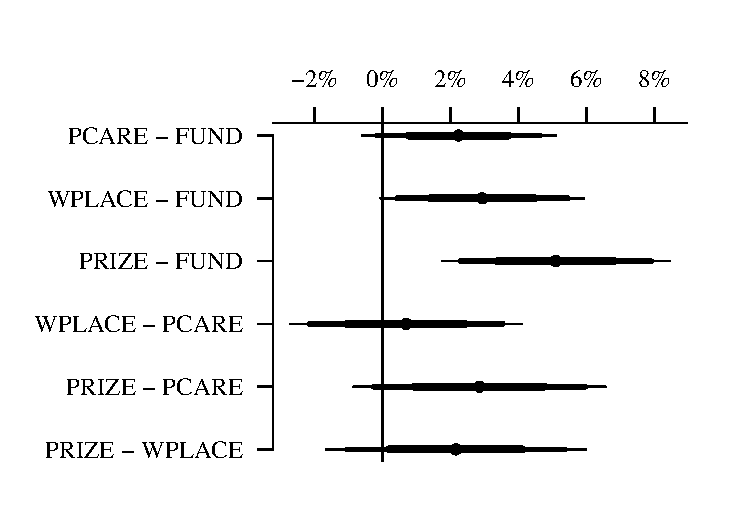
\includegraphics{Figures/cplot-1.pdf}
  \begin{tablenotes}
  This figure plots the point estimates of the difference plus $\pm 1$, $\pm 1.6$, and $\pm 2$ standard errors. Bootstrap resampling and confidence intervals based on the more conservative Holm-Bonferroni method yields very similar results (see the Appendix).
  \end{tablenotes}
\end{figure}

Results are also robust to restricting attention to staff members that
were then selected and invited by the HTL staff to submit implementation
plans for their proposals. Of the 29 workers invited to participate in
the implementation phase, most were in the PRIZE treatment (13
employees), followed by the WPLACE treatment (9 employees), the PCARE
treatment (6 employees), and the FUND treatment (only 1 employee). Also
in this case, a pairwise comparison of the probability of submitting
proposals and being selected (Figure \ref{fig: finalist}) returns a
significant and positive difference in participation between the PRIZE
and FUND treatments, as well as between the WPLACE and FUND treatments.

\begin{figure} 
  \centering
  \caption{Differences in the probability of submitting finalist project proposals}
  \label{fig: finalist}
  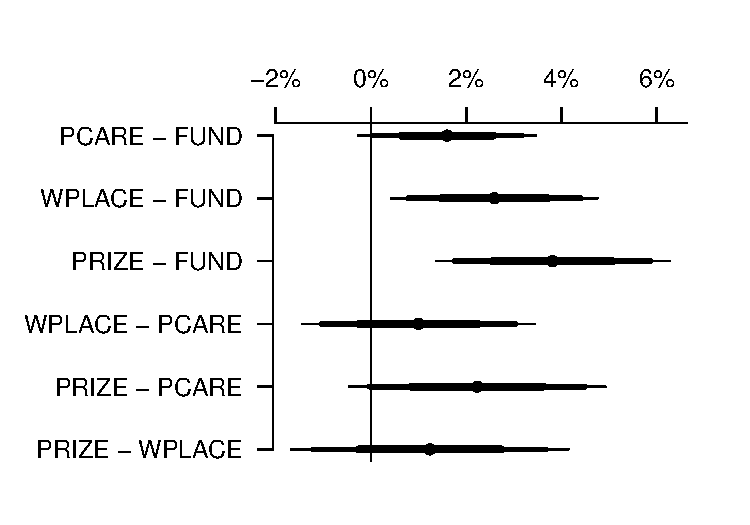
\includegraphics{Figures/cplot-2.pdf}
  \begin{tablenotes}
  This figure plots the point estimates of the difference plus $\pm 1$, $\pm 1.6$, and $\pm 2$ standard errors. Estimates have been adjusted for the small counts of finalists \citep{agresti2000simple} resulting in more conservative confidence intervals. Bootstrap resampling and confidence intervals based on the more conservative Holm-Bonferroni method yields very similar results (see the Appendix).
  \end{tablenotes}
\end{figure}

A potential concern with a causal interpretation of the above
differences lies in the possibility of \emph{contamination} among
experimental units, a topic we will discuss in greater detail in Section
\ref{discussion}. For the moment, let us point out that a
``contaminated'' sample will yield estimates of the difference in
participation biased towards zero. Intuitively, if everyone was exposed
to the content of each solicitation, participation would be the same in
each condition. Therefore, if solicitations were shared through
face-to-face communication, one should expect participation rates to
quickly converge over time. Contrary to these expectations, an analysis
of the submissions over time (Figure \ref{fig: dynamic}) does not show
signs of a strong convergence. The growth of the number of staff
submitting proposals in the PRIZE was higher in all almost weeks. Only
in the last week, participation in the WPLACE and PCARE had a little
boost. Thus, if anything, contamination occurred at the very end of the
competition. And even so, it might only have biased downwards (instead
of inflating) the estimated positive effect of prizes on participation.
In this sense, our interpretation of a large effect of prizes on
participation is robust to contamination.

\begin{figure} 
  \centering
  \caption{The dynamic of submissions}
  \label{fig: dynamic}
  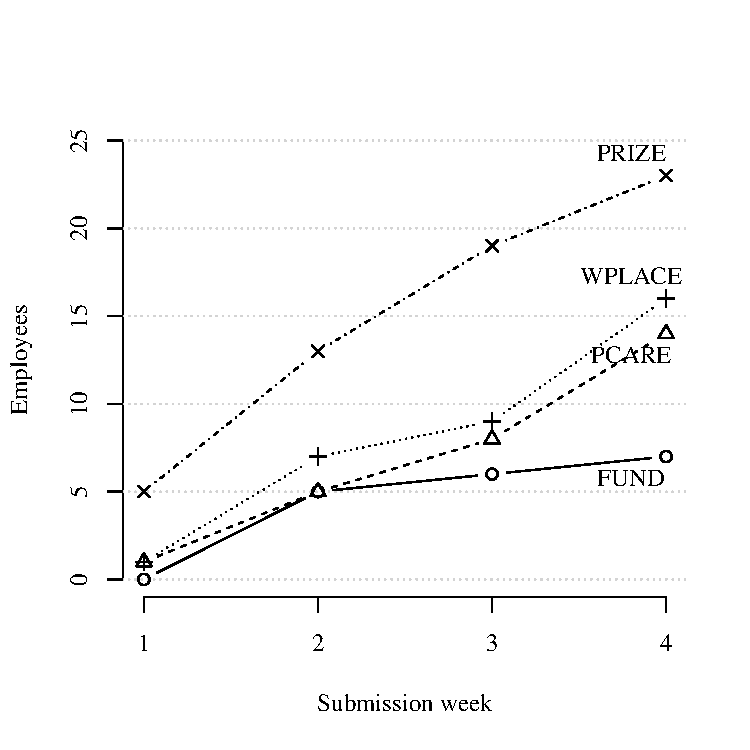
\includegraphics{Figures/dynamic-1.pdf}
  \begin{tablenotes}
  This figure plots the staff submitting proposals over the four weeks of the submission period in each condition. 
  \end{tablenotes}
\end{figure}

Although the contest was ``unbiased'' in the sense that it sought to
engage employees at all levels of the organization, one may anticipate
participation rates to vary across staff due to differences in
individual costs of participation (as our Hypothesis H5 in Section
\ref{analytical-framework-and-predictions}). To study this hypothesis,
we model the conditional probability of submitting proposals as

\begin{equation} 
  \label{eq: submit}
  \Pr(\text{SUBMIT}_{ij}) 
  = \alpha + \tau_{j} + \text{JOB}_{i} + \text{MALE}_{i} + \text{OFFICE}_{i}, 
\end{equation}

where the dependent variable \(\text{SUBMIT}_{ij}\) is 1 if the employee
\(i\) in treatment \(j\) has made a submission, and zero otherwise; the
parameter \(\tau_{j}\) denotes a change associated with the treatment
\(j\) controlling for the employee's profession (\(\text{JOB}_i\)), the
gender (\(\text{MALE}_i\)), and a dummy for office location
(\(\text{OFFICE}_i\)) that indicates whether the employee had a
permanent office instead of being assigned to a ward.\footnote{Much of
  the clinical staff might be mobile and only half of the employees
  (\(53\) percent) had fixed office locations, as they may be on duty in
  multiple wards. More senior staff tend to have a fixed location. So,
  within each profession, this measure can be viewed as a proxy for
  status inside the organization.}

\begin{table}
\centering
\caption{Probability of submitting proposals}\label{tab: probability submitting}
\begin{tabular}{@{\extracolsep{5pt}}lccccc} 
\\[-1.8ex]\hline 
\hline \\[-1.8ex] 
 & \multicolumn{5}{c}{\textit{Dependent variable:}} \\ 
\cline{2-6} 
\\[-1.8ex] & \multicolumn{5}{c}{ $SUBMIT_{ij}=1$ } \\ 
\\[-1.8ex] & (1) & (2) & (3) & (4) & (5)\\ 
\hline \\[-1.8ex] 
 PRIZE & 2.53$^{**}$ & 2.53$^{**}$ & 2.52$^{**}$ & 2.46$^{**}$ & 2.45$^{**}$ \\ 
  & (1.21) & (1.21) & (1.21) & (1.21) & (1.21) \\ 
  & & & & & \\ 
 WPLACE & 0.37 & 0.37 & 0.35 & 0.38 & 0.30 \\ 
  & (1.09) & (1.09) & (1.10) & (1.09) & (1.10) \\ 
  & & & & & \\ 
 FUND & $-$2.57$^{***}$ & $-$2.57$^{***}$ & $-$2.55$^{***}$ & $-$2.49$^{***}$ & $-$2.38$^{***}$ \\ 
  & (0.86) & (0.86) & (0.85) & (0.86) & (0.85) \\ 
  & & & & & \\ 
 Job (nursing) &  & 0.14 &  &  & 1.85 \\ 
  &  & (0.82) &  &  & (1.23) \\ 
  & & & & & \\ 
 Job (MD) &  & $-$0.31 &  &  & $-$1.14 \\ 
  &  & (1.03) &  &  & (1.24) \\ 
  & & & & & \\ 
 Male (yes) &  &  & $-$0.54 &  & $-$0.42 \\ 
  &  &  & (1.33) &  & (1.64) \\ 
  & & & & & \\ 
 Office (yes) &  &  &  & 2.79$^{**}$ & 4.56$^{***}$ \\ 
  &  &  &  & (1.20) & (1.60) \\ 
  & & & & & \\ 
 Constant & 4.84$^{***}$ & 4.78$^{***}$ & 5.00$^{***}$ & 3.35$^{***}$ & 1.97 \\ 
  & (0.61) & (0.66) & (0.73) & (0.75) & (1.25) \\ 
  & & & & & \\ 
\hline \\[-1.8ex] 
Log Likelihood & -5545 & -5545 & -5545 & -5542 & -5540 \\ 
Observations & 1,237 & 1,237 & 1,237 & 1,237 & 1,237 \\ 
\hline 
\hline \\[-1.8ex] 
\end{tabular} 
\begin{minipage}{\textwidth}
\emph{Note:} This table reports OLS estimates with heteroskedasticity robust standard errors in parenthesis. All coefficients are multiplied by 100 to indicate the percentage point change in the probability of submitting. Treatment coefficients indicate the percentage point deviation from the overall probability of submitting (there is no specific reference category). The asterisks $^{\ast\ast\ast}$, $^{\ast\ast}$, $^{\ast}$ indicate significance at 1, 5 and 10 percent level, respectively.
\end{minipage}\end{table}

Table \ref{tab: probability submitting} reports the estimation results.
To simplify interpretation, coefficients are multiplied by 100 to
indicate the percentage point change in the probability of submitting
and treatment coefficients must sum to zero to indicate deviations in
the average probability.\footnote{This is just a normalization; results
  are not affected by using a different parameterization such as using
  one treatment as a specific reference category.} First, note that
treatment differences do not change because of the individual controls,
which is reassuring given the randomization. Then, by looking at the
results of the full model (Column 5), employees in the PRIZE treatment
were 2.4 percentage points \emph{more} likely to submit compared to the
average, whereas employees in the FUND treatment were 2.4 percentage
points \emph{less} likely to do so. Subtracting these two effects gives
4.8 which is the difference in the probability of submitting between
PRIZE and FUND treatments. In a similar way, the difference in the
probability of submitting between WPLACE and FUND treatment is 2.7
percentage points, which is mildly significant (p=.083).

In columns 2 and 5, we examine effects associated with the profession of
the employee. One might expect employees to sort by profession because
differences in income between hospital employees can be sharp.\footnote{As
  mentioned before, the median wage of a physician is about 40 percent
  higher than the that of a registered nurse.} The coefficient for
nurses is indeed positive and negative for physicians, consistent with
sorting. However, these effects are not statistically different from the
residual category of other workers, as well as from one another.

In columns 3 and 5, we examine possible differential effects on
participation between men and women. Although a large literature in
economics and psychology \citep{croson2009gender} has documented a lower
propensity of women to become involved in competitive activities
\citep{niederle2007women}, we do not find evidence of such a difference.
In our setting, women are as likely as men to submit proposals.

In columns 4 and 5, we show a positive effect on participation
associated with the working having a fixed office location, as opposed
to being assigned to a ward. In our context, having a fixed office
location is highly correlated with the type of profession. For example,
nurses are more likely to being assigned to a ward than physicians or
administrative workers, due to the nature of their job. Within each
profession, however, having a fixed office location is usually
correlated with the hierarchical position inside the organization.
Hence, this variable is potentially controlling for income and
hierarchical differences occurring within each profession.

Viewing these results through our theoretical model, it appears that the
contribution cost, \(c\), may not change much between different
categories of workers. This interpretation makes sense because everyone
could have an idea on how to improve the organization, regardless of
profession or background skills. Proposals were also required to be
short and nontechnical in order to keep individual costs of
participation small for everyone. On the other hand, the cost appears
systematically lower for those with a fixed office; and one may
speculate that these are employees higher up in the hierarchy with more
experience of existing organizational problems and the available
solutions and therefore lower costs for contributing project proposals.

\subsubsection{Interactions}\label{interactions}

We now turn to examine treatment interactions involving the employee's
gender and profession.\footnote{We also look at interactions with office
  location without finding any significant difference.} Following
extensive literature on differences in preferences between men and women
\citep{croson2009gender}, gender interactions might occur as a result of
three main factors: differences in risk taking, social preferences
(willingness to contribute to public goods), and competitive
inclinations. If women prefer to work on activities that are less risky,
more pro-social (e.g., aiming at improving people's health) and where
competition is less intense, then we should observe significant
treatment interactions. Similarly, one may also expect treatment
interactions associated with the employee's profession since the
information of a fixed-value prize (i.e., the PRIZE treatment) could be
relatively less effective for employees with a higher income, such as
doctors, than the others.

\begin{figure} 
  \centering
  \caption{Differences in the probability of submitting proposals by gender and profession}
  \label{fig: interactions}
  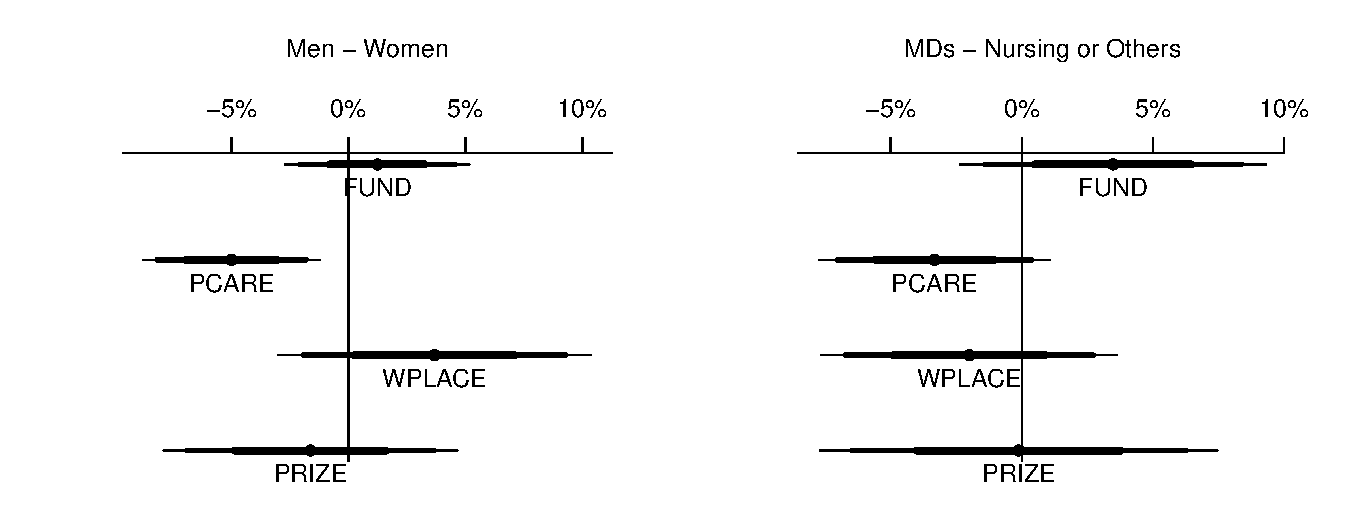
\includegraphics{Figures/plot-gender-1.pdf}
  \begin{tablenotes}
  This figure plots the point estimates of the difference between men and women (left panel) and between doctors and other workers (right panel) in each treatment plus $\pm 1$, $\pm 1.6$, and $\pm 2$ standard errors.%%Bootstrap resampling and confidence intervals based on the more conservative Holm-Bonferroni method yields very similar results (see the Appendix).
  \end{tablenotes}
\end{figure}

As shown in Figure \ref{fig: interactions} (left panel) men were
significantly less likely (about 5 percentage points) than women to
submit proposals in the PCARE treatment, while there was no gender
difference in the other treatments. Figure \ref{fig: interactions}
(right panel) also shows that there was no difference associated with
the profession: doctors are as likely to submit as any other worker in
each treatment.\footnote{As before, bootstrap resampling and the
  Holm-Bonferroni correction yields very similar results (see the
  Appendix).}

To isolate gender and profession effects, we now employ a version of
model \eqref{eq: submit} with gender-treatment interactions.\footnote{We
  also run a model with profession-treatment interactions and results
  are simular to those shown in Figure \ref{fig: interactions}.}
Estimates are shown in Table
\ref{tab: probability submitting interactions}. After gradually adding
profession and office controls, interaction coefficients remain pretty
stable across all specifications. The response of men under PCARE is
about 3 times the magnitude and in the opposite direction of the women's
response. By subtracting these two coefficients, we find a significant
difference between men and women of about 5 percentage points
(\(p=.018\)), which is consistent with our previous analysis. Thus, and
overall, we find that men responded less than women in the PCARE
treatment. This effect could be due to gender differences in preferences
and we will return on this in the discussion of the results.

\begin{table}
\centering
\caption{Probability of submitting proposals}\label{tab: probability submitting interactions}
\begin{tabular}{@{\extracolsep{5pt}}lccc} 
\\[-1.8ex]\hline 
\hline \\[-1.8ex] 
 & \multicolumn{3}{c}{\textit{Dependent variable:}} \\ 
\cline{2-4} 
\\[-1.8ex] & \multicolumn{3}{c}{ $SUBMIT_{ij}=1$ } \\ 
\\[-1.8ex] & (1) & (2) & (3)\\ 
\hline \\[-1.8ex] 
 PRIZE$\times$female & 2.99$^{*}$ & 2.95$^{*}$ & 2.84 \\ 
  & (1.68) & (1.79) & (1.78) \\ 
  & & & \\ 
 PCARE$\times$female & 1.25 & 1.21 & 1.08 \\ 
  & (1.57) & (1.61) & (1.61) \\ 
  & & & \\ 
 FUND$\times$female & $-$2.91$^{***}$ & $-$2.95$^{**}$ & $-$2.79$^{**}$ \\ 
  & (1.06) & (1.20) & (1.19) \\ 
  & & & \\ 
 WPLACE$\times$female & $-$0.49 & $-$0.52 & $-$0.62 \\ 
  & (1.35) & (1.44) & (1.43) \\ 
  & & & \\ 
 PRIZE$\times$male & 1.37 & 1.42 & 1.40 \\ 
  & (2.44) & (2.51) & (2.50) \\ 
  & & & \\ 
 PCARE$\times$male & $-$3.75$^{***}$ & $-$3.72$^{***}$ & $-$3.64$^{***}$ \\ 
  & (1.15) & (1.16) & (1.16) \\ 
  & & & \\ 
 FUND$\times$male & $-$1.67 & $-$1.65 & $-$1.48 \\ 
  & (1.70) & (1.65) & (1.66) \\ 
  & & & \\ 
 Constant & 4.80$^{***}$ & 4.79$^{***}$ & 1.87$^{*}$ \\ 
  & (0.69) & (0.70) & (1.10) \\ 
  & & & \\ 
\hline \\[-1.8ex] 
Job & no & yes & yes \\ 
Office & no & no & yes \\ 
Log Likelihood & -5542 & -5542 & -5538 \\ 
Observations & 1,237 & 1,237 & 1,237 \\ 
\hline 
\hline \\[-1.8ex] 
\end{tabular} 
\begin{minipage}{\textwidth}
\emph{Note:} This table reports OLS estimates with heteroskedasticity robust standard errors in parenthesis. All coefficients are multiplied by 100 to indicate the percentage point change in the probability of submitting. Treatment coefficients indicate the percentage point deviation from the overall probability of submitting (there is no specific reference category). The asterisks $^{\ast\ast\ast}$, $^{\ast\ast}$, $^{\ast}$ indicate significance at 1, 5 and 10 percent level, respectively.
\end{minipage}\end{table}

\subsection{Rating project proposals}\label{rating-project-proposals}

The project proposals were then rated by 178 employees (14 percent of
our sample), with the evaluators rating a median of 65.5 out of 113
project proposals (58 percent) yielding a total of 12,055
evaluator-proposal pairs.\footnote{The projects were 118 in total but,
  due to a technical problem in uploading the proposals on the website
  for evaluation, five proposals ended up with no ratings. This problem
  was independent of the treatment. A Fisher's exact test rejects any
  association between the missed proposals and the treatment of its
  proponent (\(p=.7\)).} Unlike the preceding submission phase, the
WPLACE treatment had the highest participation (Table
\ref{tab: ratings}, left panel), followed by the PCARE, the PRIZE, and
the FUND. However, using a Fisher's Exact Test for Count Data, we find
no statistically significant (p=0.339) relationship between rating
proposals and the treatments. Likewise, the differences in the count of
rated proposals (Table \ref{tab: ratings}, right panel) were not
statistically significant (a Kruskal-Wallis rank sum test gives a
p-value of 0.286). Thus, and overall, our data indicate no prolonged
effects of the treatments on both the extensive and intensive margin.
This result is consistent with the general propensity of the effects
from nudging and framing interventions to vanish over time.

One may find counterintuitive that there was less (although not
significant) participation in the evaluation phase from employees in the
PRIZE treatment than in the other treatments, given the greater
participation in the submission phase. In terms of statistical
inference, this result is not entirely surprising because only 70
percent of employees who made submissions resolved to rate proposals as
well (we detect no difference between the treatments); so, even a
difference of 2 percentage points in submitting will shrink to about 1
percentage point in the rating phase. In other words, we were not
expecting self-rating to affect evaluation much. Nevertheless, the
difference in the probability of staff rating proposals between the
PRIZE and the WPLACE or the PCARE treatments being negative might also
suggest a slight (although not significant) motivation crowding-out
effect.

\begin{table}
\centering
\caption{Outcomes of the peer evaluation phase}
\label{tab: ratings}
\begin{tabular}{@{}lcccccc}
  \\[-1.8ex]\hline \hline \\[-1.8ex]
 & \multicolumn{3}{c}{\emph{Rating proposals:}} &         \multicolumn{3}{c}{\emph{Rated proposals:}} \\
 \cmidrule(lr){2-4}\cmidrule(lr){5-7} & No & Yes & \% yes & Total & Mean & Median \\ 
  \hline \\[-1.86ex]
PRIZE & 269 & 43 & 13.8 & 2457 & 57.1 & 43 \\ 
  FUND & 272 & 36 & 11.7 & 2484 & 69.0 & 68 \\ 
  PCARE & 261 & 49 & 15.8 & 3413 & 69.7 & 73 \\ 
  WPLACE & 257 & 50 & 16.3 & 3701 & 74.0 & 82 \\ 
  [1.8ex] Total & 1059 & 178 & 14.4 & 12055 & 67.7 & 66 \\ 
   \\[-1.8ex]\hline \hline \\[-1.8ex]
\end{tabular}
\end{table}

\subsection{The quality of the project
proposals}\label{the-quality-of-the-project-proposals}

The treatment interventions may not have only impacted the propensity to
make a submission, but the quality of the submission as well. Of
particular interest is any indication of a quantity versus quality
trade-off. For example, if the FUND treatment which generated the fewest
submissions also produced the highest quality submissions. A quality
versus quantity trade-off would increase the complexity of choosing
optimal incentives for employees.

The ratings collected in the peer evaluation phase of the challenge
provide our main measure of quality. Figure \ref{fig: ratings} shows the
distribution of the ratings received by a proposal conditional on
treatment of its proponent. In each treatment, a proposal was given a
rating of 3, the ``neutral'' point, on a five-point scale about 30
percent of the times with employees being more likely to give high (4-5)
rather than low (1-2) ratings.

\begin{figure}
  \centering
  \caption{Probability of a project proposal receiving a given rating in each treatment}
  \label{fig: ratings}
  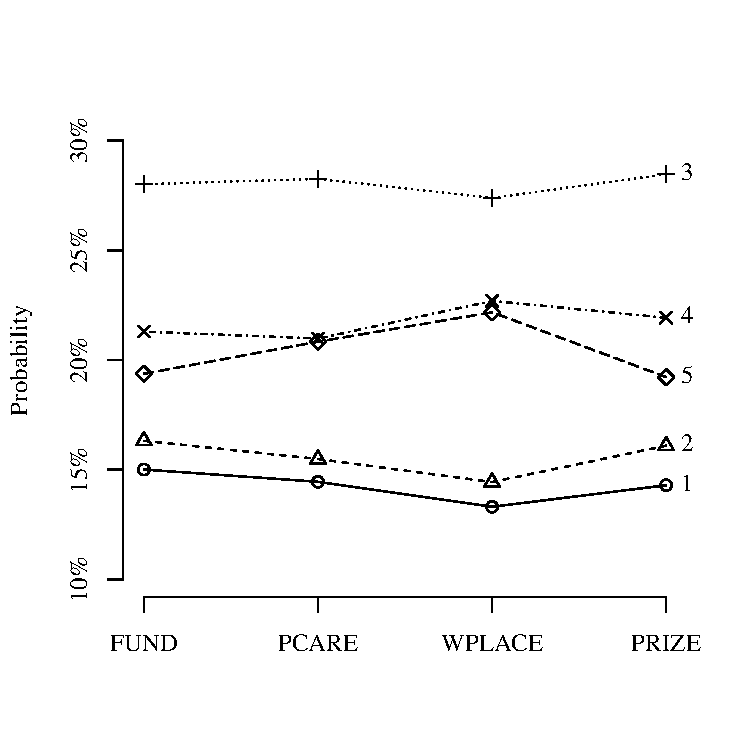
\includegraphics{figures/plot-ratings-1.pdf}
  \begin{tablenotes}
  This figure plots the distribution of the ratings given to a proposal conditional on the treatment of its proponent. Each curve presents point estimates of the probability of a project proposal receiving a given rating on a five-point scale (1=Low and 5=High). Flat, non-intersecting curves indicate that there were small differences across treatments for each rating.
  \end{tablenotes}
\end{figure}

Figure \ref{fig: ratings} reveals that the probability of a proposal
receiving a given rating was about the same in each treatment. And
indeed, by aggregating the mean rating for each proposal, we do not
identify any significant treatment effect (a Kruskal-Wallis rank sum
test gives a p-value of 0.416). Similarly, a linear regression of mean
ratings on treatment dummies does not reveal any relationship between
ratings and treatments. The treatment coefficients are not significant,
with the linear model not significantly different from a constant model
(an overall F-test gives a p-value of 0.611).

The above analysis on the aggregate ratings does not hold in general. It
crucially relies on the assumption that an increment in a proposal's
quality as measured by an increase in ratings from \(v\) to \(v+1\) is
the same for any value \(v\). So, we also examine the distribution of
ratings as generated by treatments with no aggregation. We have over
12,000 ratings, providing a very sensitive test for differences across
treatments. Using a Pearson's Chi-squared test we find that the
hypothesis of dependence between the distribution of ratings and the
treatments is \emph{not} quite significant at the 10 percent level
(p-value of 0.103). Driving the p-value is a less than \(2\) percent
difference between the proportion of 5's in the WPLACE treatment versus
the other distributions (Figure \ref{fig: ratings}), which is probably
due to outliers (the winning proposal was in the WPLACE treatment).
Taken together with the fact that our sample is large, we have strong
evidence suggesting that there are no (economically meaningful)
differences in the quality of project proposals across treatments and in
particular no evidence of a quantity versus quality trade-off up to the
resolution of the five-point scale.\footnote{One may worry that such
  binning is a fairly coarse measure of quality. In particular, effects
  concentrated in the upper tail of the distribution may not be
  detected. For example, compare the ratings of proposals A, B, C and D
  with hypothetical true qualities of 3, 4, 5, and 10 stars
  respectively. Under a five-point scale rating system, proposals A and
  B can be distinguished, but C and D cannot be distinguished. Hence,
  one needs to be very cautious in interpreting these results as
  evidence against quality effects in general.}

One potential limit of assessing quality only on the basis of peer
ratings is that the employees might have a different view of a
proposal's quality than executives (due, for instance, to a misalignment
of incentives). And indeed, to ensure alignment between managerial goals
and the peer assessment, all project proposals were further vetted by
the HTL staff before being considered for implementation funding. So, we
now focus on the outcomes of this vetting process to investigate more
broadly the presence of treatment effects on the quality of project
proposals.

The vetting process conducted by the HTL staff resulted in 93 proposals
being scored (from 1 to 100 points) with the best 29 proposals invited
to submit implementation plans. The remaining 20 proposals were excluded
(and received a score of zero) either because flagged as inappropriate
for funding or because the proponent manifested intention to not
participate in the implementation phase (a Fisher's Exact Test for Count
Data finds no association between proposals excluded and treatments with
a p-value of 0.652).

The Spearman's rank correlation coefficient between the scores given by
the HTL staff and the average peer ratings was relatively high (0.198),
indicating good agreement between our two measures of quality. Indeed,
as before, we find no treatment effects on quality using the scores (a
Kruskal-Wallis rank sum test gives a p-value of 0.437). We also find no
treatment differences in the percentage of submitters being selected and
invited by HTL staff to present additional implementation plans (a
Fisher's Exact Test for Count Data gives a p-value of 0.652). Although
not significant, employees who made project proposals in the FUND
treatment were less likely to be selected as finalist than the others
(only 1 out of 7 in the FUND treatment were selected and invited by the
HTL staff), providing additional evidence of a no quantity versus
quality trade-off, as discussed before.

\subsection{The content of the project
proposals}\label{the-content-of-the-project-proposals}

The goal of the challenge was to improve Heart Center operations by
identifying problem areas and potential solutions. The proposed projects
broadly conformed to the stated goals of the contest, aligning with
improving the work processes within the organization or providing
high-quality patient care. For example, one project proposal that
received high peer ratings was to create a platform for patients to
electronically review and update their med list in the office prior to
seeing the physician. Another was to develop a smartphone application
that allows the patient to see the itinerary for the day providing a
guide from one test or appointment to another. Nevertheless, other
contest organizers may have varying goals and be concerned about
different aspects of the submissions. In order to examine additional
dimensions of submission content, we now study the area of focus of the
submissions. Of particular interest is understanding whether the framing
intervention induced employees to concentrate on different categories.
For example, while staff in the WPLACE treatment focused on improvements
for the workplace, those in the PCARE treatment concentrated on
interventions directly targeting the patients.

\begin{table}
\centering
\caption{Project proposals by area of focus}
\label{tab: area-of-focus}
\begin{tabular}{@{}lccccc}
  \\[-1.8ex]\hline \hline \\[-1.8ex]
 & FUND & PCARE & WPLACE & PRIZE & Total \\ 
  \hline \\[-1.86ex]
Information and access & 0 & 4 & 8 & 11 & 23 \\ 
  Patient support & 2 & 8 & 7 & 6 & 23 \\ 
  Care Coordination & 1 & 9 & 3 & 7 & 20 \\ 
  Staff workflow & 4 & 5 & 4 & 5 & 18 \\ 
  Workplace & 3 & 6 & 3 & 5 & 17 \\ 
  Quality and safety  & 0 & 0 & 5 & 5 & 10 \\ 
  Surgical tools and support to research & 1 & 1 & 0 & 0 & 2 \\ 
  [1.8ex] Total & 11 & 33 & 30 & 39 & 113 \\ 
   \\[-1.8ex]\hline \hline \\[-1.8ex]
\end{tabular}
\begin{tablenotes}
The areas of focus were manually identified by the HTL staff at the end of the competition. Due to a technical problem five proposals ended up with no classification.
\end{tablenotes}
\end{table}

Members of the HTL categorized each project proposal into one of seven
``areas of focus'' (Table \ref{tab: area-of-focus}): three categories
(``Care coordination'', ``Staff workflow'', ``Workplace'') identified
improvements for the workplace, other three (``Information and access'',
``Patient care'', and ``Quality and Safety'') focused on improvements
centered around patients, and another one (``Surgical tools and support
to research'') categorized projects developing tools to support
scientific research.

Using a Fisher's Exact Test for Count Data with simulated p-value (based
on 50000 replicates), we find a mildly significant (p=0.089) association
between these categories and the treatments.\footnote{Simulations are
  used to reduce the computational burden.} The analysis of pairwise
differences between treatments (Figure \ref{fig: areas of focus})
reveals that this result is driven by differences in the ``Quality and
Safety'' and ``Information and access'' categories. Project proposals in
the PCARE treatment were less likely to fall in the ``Quality and
Safety'' category. Similarly, project proposals in the FUND treatment
were less likely to fall in the ``Information and access'' category.\\
It is difficult to interpret these effects because our model does not
provide any prediction on the content of proposals. One possibility is
that framing induced participants to concentrate on different areas of
interventions but our data do not appear consistent with this story.

\begin{figure}
  \centering
  \caption{Differences in the probability of proposals being in a given area of focus in each treatment}
  \label{fig: areas of focus}
  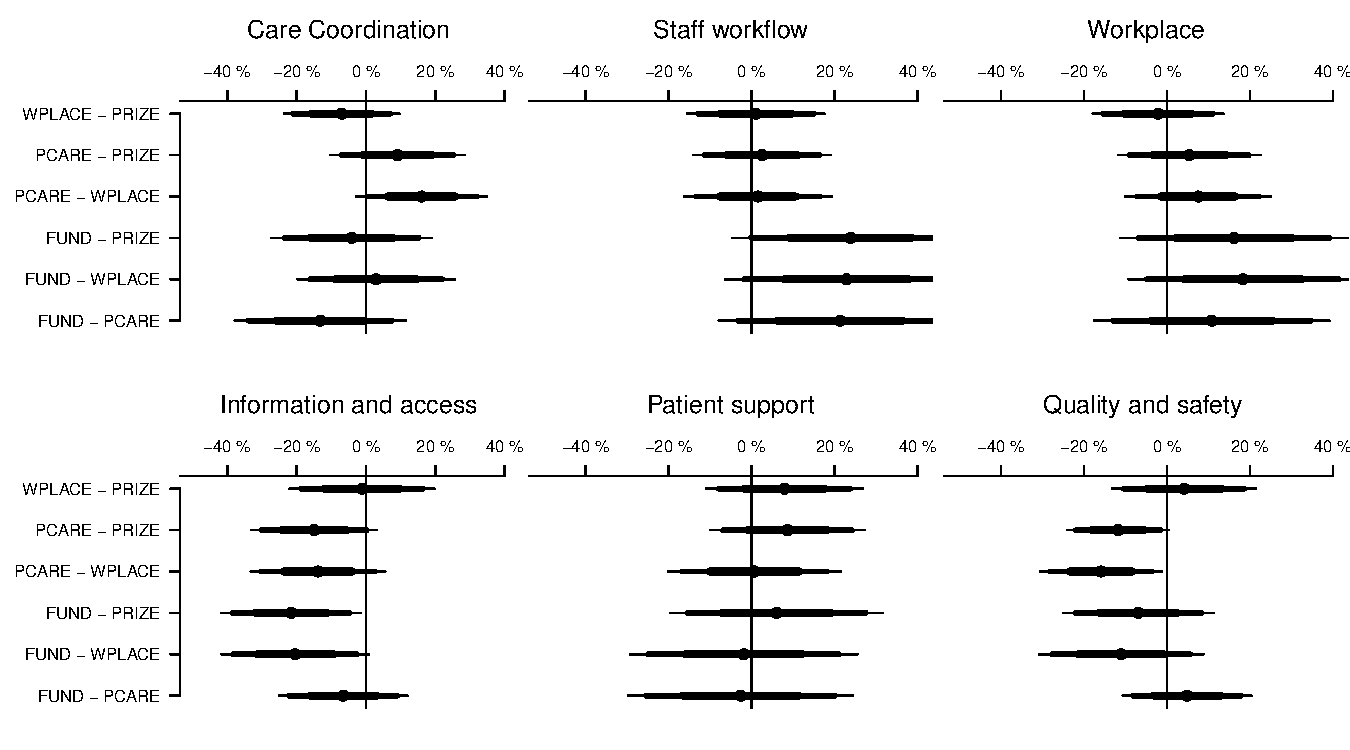
\includegraphics{figures/areas-1.pdf}
  \begin{tablenotes}
  This figure plots the point estimates of the difference plus $\pm 1$, $\pm 1.6$, and $\pm 2$ standard errors. Estimates have been adjusted for the small counts of the data \citep{agresti2000simple} resulting in more conservative confidence intervals.
  \end{tablenotes}
\end{figure}

Another possibility is that of differences in the underlying complexity
of the project proposal that were not captured by our measure of
quality. To address this issue, we now turn to examine differences in
the length of a proposal as measured by the word count of a submission.
Submissions were below 200 words in most cases with little differences
between the treatments. Indeed, testing for a significant linear
regression relationship between the length of submissions and treatment
dummies returned an overall insignificant result (p=.43, F-test).

As a result, based on the analysis of the areas of focus and the length
of the submissions, we do find only little evidence of differences in
submission content across treatments. However, submission content is not
a well-defined concept and could be characterized in many dimensions.
While content does not vary in the dimensions we selected, we have not
exhausted all possible dimensions.

\subsection{Estimating social
preferences}\label{estimating-social-preferences}

In this section, we calibrate the theoretical model developed in Section
\ref{analytical-framework-and-predictions} with the experimental data to
get a sense of the magnitude of underlying preferences for contributing
to the organization. Following, the mixed-strategy equilibrium of the
model, the theoretical probability of contributing must be proportional
to the expected value of winning, \(R\), the underlying preferences
towards the public good, \(\gamma\), the marginal costs of contributing,
\(c\), and the number of agents, \(n\).

We assume the cost of making a submission \(c\) is the same in each
treatment,\footnote{This seems a reasonable assumption, given everyone
  is asked to perform the same task (identical submission procedure,
  same word limit, etc.).} and the individual preferences are constant,
being predetermined to our intervention. Then we derive a structural
relationship between the observed difference in the probability of
contributing \(\Delta p\) and the difference in the expected rewards
from winning \(\Delta R\) between the treatments.That is,\footnote{This
  equation can be obtained by following these steps. First, we
  approximate the profit equating condition \eqref{eq: mixed-strategy}
  to a linear function by noticing that the \(1/(1-(1-p)^n)\)
  approximates one for \(n\) large enough and \(p\) sufficiently small.
  Second, we solve for \(p\) and we simplify using the definitions of
  \(\Delta p\) and \(\Delta R\).}

\begin{equation}
  \Delta p \approx\frac{\Delta R}{n (c - \gamma)}.
\end{equation}

(Throughout this section we will consider \(\delta=0\) ignoring the
distinction between impure and pure altruism.) By solving for
\(\gamma\), we get

\begin{equation}
  \label{eq: gamma}
  \gamma   \approx  c -  \Delta R / (n\Delta p). 
\end{equation}

This implies that the parameter capturing individual preference for the
public good (that is consistent with our data) must be proportional to
the ratio between the difference in rewards and the difference in the
probability of submitting. Although we do not observe the levels of
\(R\) in each treatment, we approximate the difference of rewards
between the PRIZE and the other conditions by the pecuniary value of the
reward, which has its upper bound in the highest price that can be paid
for an iPad mini (\$350).\footnote{The price paid by the Heart Center
  was \$239 at the end of 2014 (including shipping cost). Other popular
  models (those with cellular data and large storage) could cost as high
  as \$350. Agents, however, were not aware of the specific model used
  for the competition and of the price paid. So, the value of \$350 is
  very conservative.} We further calibrate the cost of submitting a
proposal \(c\) to \$40 which is the median income per hour of a Nurse
Practitioner according to the Bureau of Labor Statistics; we assume the
number of competitors \(n\) to be 30 percent of the entire sample to
take into account rational expectations about the actual number of
participants in the contest.\footnote{This choice is our best guess of
  the number of active staff members at the Heart Center and is based on
  the number of employees who voluntarily took a survey before the
  experiment (378 people). Assuming greater participation would lead to
  artificially increasing the estimates of underlying incentives. In
  fact, staff members may have rational expectations about the actual
  number of potential participants, which may be less than the entire
  population.} Finally, by substituting these calibrated values into
equation \eqref{eq: gamma} along with the empirical difference in
participation rates between the PRIZE and the other treatments
(\(\Delta p=0.037\)), we get an estimate of the magnitude of the social
preferences towards the organization which is \(\hat\gamma=\$12\). As
shown in Figure \ref{fig: gamma}, this value is equivalent to about 30
percent reduction in the cost of contributing. Hence, increasing the
prize by \$100 is expected to raise the probability of submitting by 1
percentage points. This increase can be compared to the corresponding
increase of 0.7 that one will obtain by assuming no social preferences
\(\gamma=0\) at all.

\begin{figure} 
\centering
\caption{Estimated value of social preferences ($\hat\gamma$)}
\label{fig: gamma}
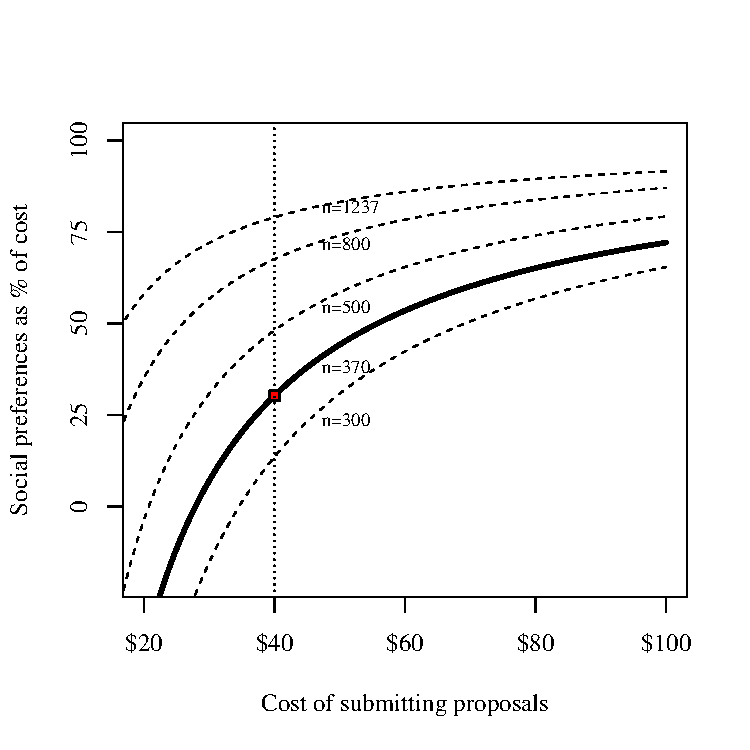
\includegraphics{figures/gamma-1.pdf}
\begin{tablenotes}
This figure plots the theoretical relationship between the cost of participation and the the social preferences parameter $\gamma$ (in percentage of the costs) which is consistent with our experimental data. Different curves represents different assumptions on the number of competitors. 
\end{tablenotes}
\end{figure}

A few remarks are in order here. To get confidence around these
estimates one need to consider several sources of uncertainty. First,
there is the uncertainty of estimating the probability of submitting in
our sample (standard errors can be computed directly from the data).
Another source of uncertainty is due to the calibration of the marginal
cost or the number of competitors. As shown in Figure \ref{fig: gamma},
the fraction of costs explained by social preferences increases
monotonically in the number of competitors (going up to 80 percent of
costs if employees expected to compete against every Heart Center staff
member); and decreases monotonically in the calibrated cost of making a
submission. Finally, another important source of uncertainty is
regarding the main behavioral assumptions of the model, as we discuss in
the next section.

\section{Discussion}\label{discussion}

In this article, we report the results of a natural field experiment
conducted during an innovation contest held in a medical center with
over 1200 employees. Different incentives for participation were
announced by manipulating the personal messaging to employees. Messaging
emphasized either available prizes (iPad mini's) for top submissions,
motives for improving patient care and improving the workplace, or a
funding opportunity alone. Our data show that announcing a relatively
small prize for top submissions boosted employee participation by 85
percent without affecting the quality of the submissions. The effect was
the same for men and women, workers with high and low-income levels, and
appears too large to fit a pure contest environment without public good
incentives. Our interpretation is that participation was driven by a
complementarity between prizes and mission-oriented preferences towards
improving the organization. Using a simple model, we estimate that these
preferences can explain about 25 percent of the magnitude of the effect.

One objection to this interpretation is that employees could have had
ulterior motivations to take part in the innovation contest. Common
factors are the prospect of a promotion and career advancement
\citep{baker1994internal, gibbs1995incentive} or to earn professional
prestige and peer recognition
\citep{kosfeld2011getting, blanes2011tournaments}. While these other
factors are important and could have influenced overall participation
levels, these do not seem to explain well our findings. First, the
incentive to gain a career promotion was only marginal but even assuming
that employees viewed winning the innovation contest as a good chance to
advance their career, our messaging intervention was fairly neutral to
any potential career opportunities associated with the challenge. So, it
does not explain well our finding of significant differences between
treatments. The same goes for the opportunity of a recognition, which is
possibly a more plausible alternative explanation for participation.
Also, in this case, it is hard to imagine how the messaging could create
different reputation incentives that appear instead associated with
actions that were the same in each treatment, such as the HTL announcing
the winners during a public event at MGH and/or publishing their names
on the website of the organization.

Another concern is with ``contamination'' or ``interference'' between
experimental units. This situation is problematic as it violates the
Stable Unit Treatment Value Assumption (SUTVA) for causal inference
\citep{rubin1974estimating}. With contamination, for instance, decisions
of one staff member depend on its treatment and on the treatments of
others, such as its neighbors. This may lead to a bias that depends on
the level of interference (how intense is the communication among
subjects) but also on the association between individual and
neighborhood treatments (how dense is the network of social
interactions). Despite this problem can seriously bias our estimates, we
know the direction of the bias. Because communication would spread the
content of the messaging across treatments, we should expect
participation differences to converge to zero (a bias towards a null
effect). When the information is the same for everyone, participation
rates should be on average the same in each condition. So, if one does
not believe the SUTVA holds, our finding significant differences between
treatments can still be interpreted in the sense of a lower bound of the
true effect. Even so, internal communication during the submission phase
was likely small: staff members competing against one another had only
weak incentives for information sharing. Furthermore, we find little
evidence of a converge when we examine the dynamic of participation.
Hence, and overall, even if there was a bias due to contamination one
should expect such bias to be small.

One might also worry that employees had a poor understanding of the
costs from winning the contest which may explain the participation
effects. An empirical regularity in laboratory experiments on contests
\citep[see][]{dechenaux2014survey} is that people are likely to make
mistakes, which may lead to higher effort levels than predicted. Here, a
serious concern is that employees in the PRIZE treatment underestimated
the costs of taking part in the implementation phase. Announcing prizes
may have made more salient the immediate rewards (the iPad's) inducing
employees to pay less attention to the costs of being involved in
implementing their own project. If so, some of those who submitted
proposals in the PRIZE treatment would reconsider their choice as the
competition moved to the implementation phase. Instead, we find that
only a negligible fraction of employees submitting proposals was not
responsive to the invitation or declined participation in the
implementation phase; a behavior that was not different across
treatments. Hence, although employees might have had incorrect beliefs
or systematic biases that lowered expected costs from winning, these are
unlikely to explain the observed significant differences.

Another finding that deserves further comment is that responses were
sensitive to the gender of the solicited person. Indeed, women's
participation was greater than men's when emphasizing the patient care
mission, controlling for the profession. This result echoes
\citet{delfgaauw2013tournament} showing gender differences in a sales
contest associated with the way a competition is announced or
``framed.'' This finding is open to various interpretations. One
possibility is that female workers may be more altruistic or perceive
the mission of the organization differently than male workers. However,
the existing literature in economics \citep{croson2009gender} is not
unanimous on this point. Another possibility is that workers were
affected in their submission decisions by self-stereotypes associated
with the framing condition. Gender-based stereotypes are indeed
pervasive in healthcare organizations \citep{evans2002cautious}. So one
may speculate that men's propensity to participate was lower in
activities perceived as female-typed. In this sense, our study is
related to \citet{coffman2014evidence} who finds evidence in the
laboratory that women are less likely to contribute ideas to groups when
the topic falls in male-typed domains, e.g., sports, and vice versa.

An interesting (non-)finding is the lack of gender-based differences
with respect to participation in the prize (PRIZE) treatment where
women's participation was equal to men's. An extensive literature in
economics has shown significant gender differences in preferences women
concerning risk-aversion \citep{borghans2009gender} and women's distaste
for competition compared to men \citep{niederle2007women}. So, one may
be concerned that using a contest incentive structure to encourage the
private provision of a public good would discourage participation by
women. In our experiment, by contrast, women participated most in the
treatment emphasizing the contest prize suggesting that this type of
contest is robust to these effects. This result could be driven by some
unique characteristics of our subject pool (healthcare professional
workers), the exploration of which is beyond the scope of the present
study.

Another key aspect of our study is the possibly negative interaction
between reward incentives and the mission-oriented motivation to
contribute. A \emph{negative interaction} occurs when incentives
crowd-out the motive to contribute. Crowding out effects have been seen
in other experiments in the context of blood donations
\citep{lacetera2013economic, lacetera2014rewarding}, or the crowding in
effects seen with public ``bads'' in daycare pick-ups
\citep{gneezy2000fine}. We do not observe evidence of a crowding-out in
our environment, but differences in context make comparisons difficult.
Pecuniary incentives may not have the same effect if in-kind gifts are
used in place of currency \citep[e.g.,][]{kube2012currency}, or if the
setting already involves an employer-employee relationship
\citep[e.g.,][]{fehr1998gift}.

Finally, while the choice of focusing on healthcare workers may limit
the generality of our results in some respect, it should be noted that
in the US alone health care spending accounts for 17 percent of the GDP
(in 2015) and, more generally, our study results are also directly
applicable to a variety of other professions exposed to a public good
dilemma (e.g., teachers, public servants, researchers).

In conclusion, the results presented here have implications that go
beyond the specific organization under study. Using a competition for
prizes appears a profitable way for firms to encourage contributions
among workers in situations resembling a private provision of public
goods. In many settings, this approach can be more effective than what
is acknowledged in the traditional tournament theory literature. The
reason being that the incentive effect of prizes interacts with
prosocial motivations of workers to exert effort. The management can
appeal to internal motivations towards the mission of the organization
to raise the level of voluntary contributions. However, this may be
tricky in practice due to the heterogeneity of motivated agents. In
particular, the evidence on gender differences in response to framing
suggests female workers may perceive the goals of the organization
differently from male workers. Investigating the causes of these
gender-based differences is left as an avenue for future research.

\renewcommand\refname{References}
\bibliography{library.bib}

\end{document}